%%%%%%%%%%%%%%%%%%%%%%%%%%%%%%%%%%%%%%%%%%%%%%%%%%%%%%%%%%%%%%%%%%%%%%%%%%
% CircuitWithOneTransistorAndOneLoadResistor
%%%%%%%%%%%%%%%%%%%%%%%%%%%%%%%%%%%%%%%%%%%%%%%%%%%%%%%%%%%%%%%%%%%%%%%%%%

\newcommand{\figCircuitWithOneTransistorAndOneLoadResistor}
{
    \begin{figure}[htb]
        \begin{center}
            \begin{circuitikz}[european currents,european resistors,american inductors]
                \draw
                (0,0) coordinate(U+) to [short,-] ++(0.5,0)  
                node[currarrow](Tl){} -- ++(1,0) ++(0.5,0) node[nigfete,rotate=90](Trans){} -- ++(1.5,0) coordinate(Tr)
                    to [short,-*] ++(0.5,0) coordinate(junc1)   -- ++(0.5,0) coordinate(Ll) to [L,l_=$L$,i^=$i_\text{L}$]
                    ++(2,0) coordinate(Lr) to [short,-*] ++(0.5,0) coordinate(junc2)  -- ++(2,0)
                    coordinate(Rt) to [R,l_=$R$,i_=$i_\text{2}$,v^=$U_\text{2}$,voltage shift=0.5, voltage=straight] ++(0,-3) coordinate(Rb)
                    to [short,-*] ++(-2,0) coordinate(junc3) to [short,-*] ++(-3,0) coordinate(junc4) to [short] ++(-2,0)
                    coordinate(junc5) to [short,-] ++(-2,0) coordinate(U-)
                    (junc2) to [C,l_=$C$](junc3)
                    (junc4) to [short]  ++(0,0.5) coordinate(Db) to[D-,l^=$D$]  ++(0,2) coordinate(Dt) to [short] (junc1)
                    (Trans.G)  to [sqV] ++(0,-1)(junc5) 
                
                (U+) to [V=$U_1$] (U-)
                
                (Trans)  node[anchor=south,color=black]{$T_1$}	
                (Tl)  node[anchor=south,color=black]{$i_\text{1}$}	
                ;
            \end{circuitikz}
        \end{center}
        \caption{Circuit with one transistor, filter and one load resistor.}
        \label{fig:step_down_converter_output_filter}
    \end{figure}
}

%%%%%%%%%%%%%%%%%%%%%%%%%%%%%%%%%%%%%%%%%%%%%%%%%%%%%%%%%%%%%%%%%%%%%%%%%%
% StepDownConverterOutputFilter
%%%%%%%%%%%%%%%%%%%%%%%%%%%%%%%%%%%%%%%%%%%%%%%%%%%%%%%%%%%%%%%%%%%%%%%%%%

\newcommand{\figStepDownConverterOutputFilter}
{
    \begin{figure}[htb]
        \begin{center}
            \begin{circuitikz}[european currents,european resistors,american inductors]
                \draw
                (0,0) coordinate(U+) to [short,-] ++(0.5,0)  
                node[currarrow](Tl){} -- ++(1,0) ++(0.5,0) node[nigfete,rotate=90](Trans){} -- ++(1.5,0) coordinate(Tr)
                    to [short,-*] ++(0.5,0) coordinate(junc1)   -- ++(0.5,0) coordinate(Ll) to [L,l_=$L$,i^=$i_\text{L}$]
                    ++(2,0) coordinate(Lr) to [short,-*] ++(0.5,0) coordinate(junc2)  -- ++(2,0)
                    coordinate(Rt) to [R,l_=$R$,i_=$i_\text{2}$,v^=$U_\text{2}$,voltage shift=0.5, voltage=straight] ++(0,-3) coordinate(Rb)
                    to [short,-*] ++(-2,0) coordinate(junc3) to [short,-*] ++(-3,0) coordinate(junc4) to [short] ++(-2,0)
                    coordinate(junc5) to [short,-] ++(-2,0) coordinate(U-)
                    (junc2) to [C,l_=$C$](junc3)
                    (junc4) to [short]  ++(0,0.5) coordinate(Db) to[D-,l^=$D$]  ++(0,2) coordinate(Dt) to [short] (junc1)
                    (Trans.G)  to [sqV] ++(0,-1)(junc5) 
                
                (U+) to [V=$U_1$] (U-)
                
                (Trans)  node[anchor=south,color=black]{$T_1$}	
                (Tl)  node[anchor=south,color=black]{$i_\text{1}$}	
                ;
            \end{circuitikz}
        \end{center}
        \caption{Circuit with one transistor, filter and one load resistor.}
        \label{fig:step_down_converter_output_filter}
    \end{figure}
}

%%%%%%%%%%%%%%%%%%%%%%%%%%%%%%%%%%%%%%%%%%%%%%%%%%%%%%%%%%%%%%%%%%%%%%%%%%
% BuckConverterWithOneTransistorAndOneDiode
%%%%%%%%%%%%%%%%%%%%%%%%%%%%%%%%%%%%%%%%%%%%%%%%%%%%%%%%%%%%%%%%%%%%%%%%%%


\newcommand{\figBuckConverterWithOneTransistorAndOneDiode}
{
    \begin{figure}[ht]
        \begin{center}
            \begin{circuitikz}[european currents,european resistors,american inductors]
                \draw
            (0,0) coordinate(N1) to [short] ++(1.5,0) coordinate(Ud)
            ++(0,-1) node[nigfete](Trans){}
            (Ud) to [short,i=$i_{\mathrm{c}}(t)$] (Trans.drain)
            (Trans.source) to [short,-] ++(0,0) coordinate(U2p)
            node[circ]{}
            to [short,-] ++(0,0) to [L,l^=$L$] ++(3,0) coordinate(Lp) to [short,-] ++(0,-2) coordinate(Lp10)
            (Lp) to [V, v_=$U_2$] (Lp10)
            (Lp) to [open] (Lp10)
            coordinate(Lp10) to  [short,-] ++(-3,0) coordinate(D)
            to [D,l^=$D$, i=$i_{\mathrm{D}}(t)$] ++(0,2)
            (0,-3.77) coordinate(Bw) to [short] ++(3,0) coordinate(U1)
            %(N1) to [V] (Bw)
            (N1) to [V,v_=$U_1$] (Bw)
            ;
            \end{circuitikz}
        \end{center}
        \caption{Buck converter with one transistor and one diode.}
    \end{figure}
}

%%%%%%%%%%%%%%%%%%%%%%%%%%%%%%%%%%%%%%%%%%%%%%%%%%%%%%%%%%%%%%%%%%%%%%%%%%
% SwitchOnBehaviorAndSwitchOffBehaviorOfUI
%%%%%%%%%%%%%%%%%%%%%%%%%%%%%%%%%%%%%%%%%%%%%%%%%%%%%%%%%%%%%%%%%%%%%%%%%%

\newcommand{\figSwitchOnBehaviorAndSwitchOffBehaviorOfUI}
{
    \begin{figure}[ht]
        \centering
        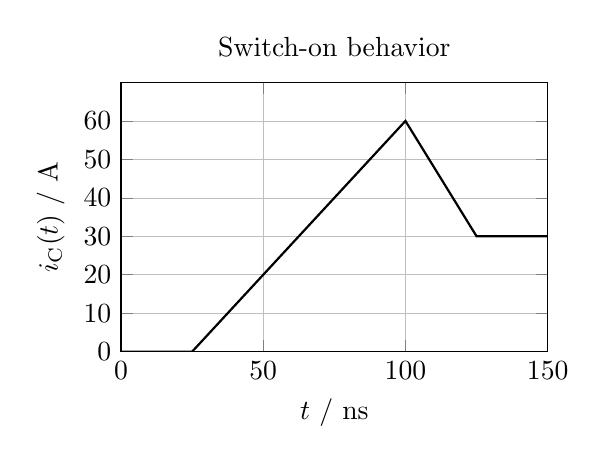
\begin{tikzpicture}
        \begin{axis}[
            width=7cm, height=5cm,
            grid=both,
            major grid style={line width=.2pt,draw=gray!50},
            minor grid style={line width=.1pt,draw=gray!20},
            xlabel={$t$ / ns},
            ylabel={$i_\mathrm{C}(t)$ / A},
            title={Switch-on behavior},
            xmin=0, xmax=150,
            ymin=0, ymax=70,
            xtick={0, 50, 100, 150},
            ytick={0, 10, 20, 30, 40, 50, 60},
            ]
            % Einschaltverhalten graph
            \addplot[
                thick,
                mark=none,
                color=black,
            ] coordinates {
                (0,0) (25,0) (50, 20) (75, 40) (100, 60) (125, 30) (150, 30)
            };
        \end{axis}
        \end{tikzpicture} 
        \hspace{1cm} % Abstand zwischen den beiden Diagrammen
        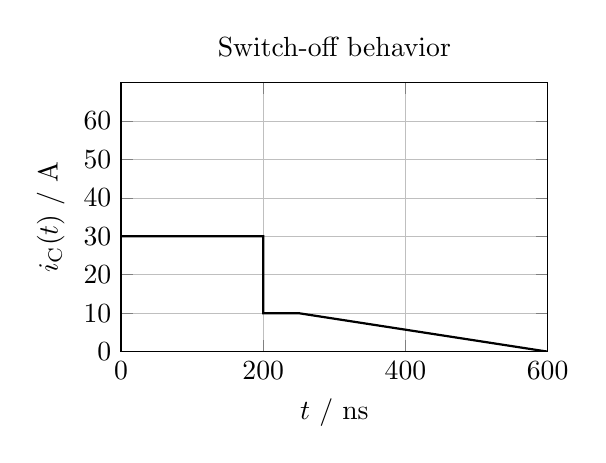
\begin{tikzpicture}
        \begin{axis}[
            width=7cm, height=5cm,
            grid=both,
            major grid style={line width=.2pt,draw=gray!50},
            minor grid style={line width=.1pt,draw=gray!20},
            xlabel={$t$ / ns},
            ylabel={$i_\mathrm{C}(t)$ / A},
            title={Switch-off behavior},
            xmin=0, xmax=600,
            ymin=0, ymax=70,
            xtick={0, 200, 400, 600},
            ytick={0, 10, 20, 30, 40, 50, 60},
            ]
            % Ausschaltverhalten graph
            \addplot[
                thick,
                mark=none,
                color=black,
            ] coordinates {
                (0,30) (200, 30) (200, 10) (250, 10) (600, 0)
            };
        \end{axis}
        \end{tikzpicture}
        \caption{Switch-on behavior and switch-off behavior of $i_{\mathrm{C}}(t)$}
        \label{fig:Switch-on behavior and switch-off behavior of}
    
        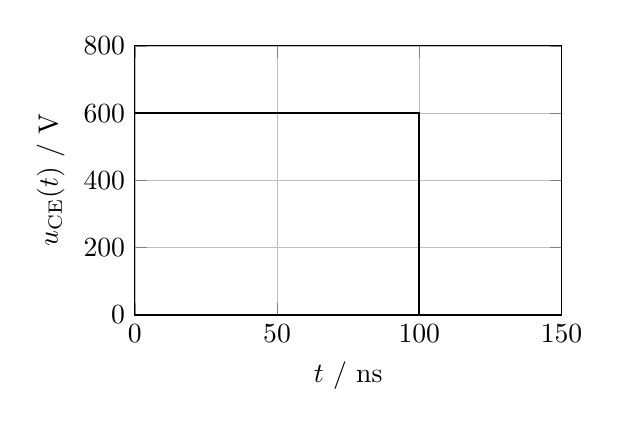
\begin{tikzpicture}
        \begin{axis}[
            width=7cm, height=5cm,
            grid=both,
            major grid style={line width=.2pt,draw=gray!50},
            minor grid style={line width=.1pt,draw=gray!20},
            xlabel={$t$ / ns},
            ylabel={$u_{\mathrm{CE}}(t)$ / V},
            xmin=0, xmax=150,
            ymin=0, ymax=800,
            xtick={0, 50, 100, 150},
            ytick={0,200, 400, 600, 800},
            ]
            % Einschaltverhalten graph
            \addplot[
                thick,
                mark=none,
                color=black,
            ] coordinates {
                (0,600) (100, 600) (100, 0)
            };
        \end{axis}
        \end{tikzpicture}
        \hspace{1cm} % Abstand zwischen den beiden Diagrammen
        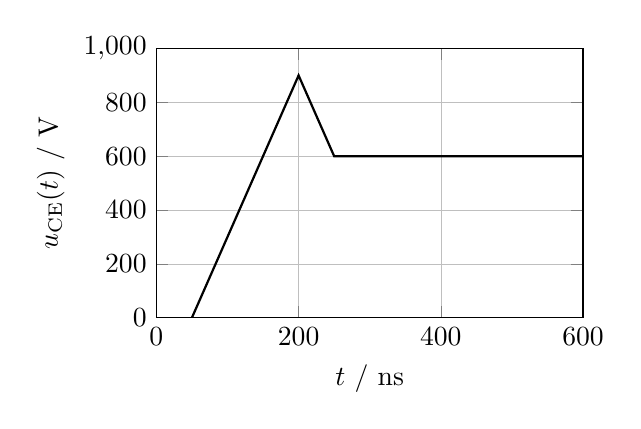
\begin{tikzpicture}
        \begin{axis}[
            width=7cm, height=5cm,
            grid=both,
            major grid style={line width=.2pt,draw=gray!50},
            minor grid style={line width=.1pt,draw=gray!20},
            xlabel={$t$ / ns},
            ylabel={$u_{\mathrm{CE}}(t)$ / V},
            xmin=0, xmax=600,
            ymin=0, ymax=1000,
            xtick={0,200, 400, 600},
            ytick={0,200, 400, 600,800, 1000},
            ]
            % Ausschaltverhalten graph
            \addplot[
                thick,
                mark=none,
                color=black,
            ] coordinates {
                (50,0) (200, 900) (250, 600) (600, 600)
            };
        \end{axis}
        \end{tikzpicture}
        \caption{Switch-on behavior and switch-off behavior of $u_{\mathrm{CE}}(t)$.}
        \label{fig:Switch-on behavior and switch-off behavior of voltage}
    \end{figure}
}
